本章首先将介绍本文的核心方法——图神经网络,接着介绍推荐系统是怎样更好地利用图神经网络的。最后本章提出轻量化的社会标注图协同过滤模型 (Light Folksonomy Graph Collaborative Filtering, LFGCF) 的设计。

\section{图神经网络}
本节将介绍图神经网络的一般形式。初始设定的图神经网络通常用于进行节点分类、整图分类等任务。如何合理的调整模型的组件是图神经网络在推荐系统应用的研究重点与热点。
\subsection{针对图表征学习的图神经网络}
近年来,深度学习在处理符合欧氏结构(euclidean structure)的数据类型,如图片和文本等方面取得了显著的成果。这些数据通常被视为高维张量(Tensor)进行处理,具有信息量丰富、结构稠密等特点。然而,在实际场景中,非欧式结构(non-euclidean structure)的数据类型却更加普遍,其中最常见的便是图数据。推荐系统中的数据就包含大量的图数据,例如由大量用户和物品组成的用户-物品二部图、用户与用户之间的社交网络以及物品与物品之间的实体关系知识图谱等。这些数据通常是极度稀疏的,这使得深度学习模型在推荐系统领域并没有很快取代传统算法。而图神经网络的出现,则有效地解决了这一窘境\cite{wu_survey_2022}。

随着图数据的广泛应用,图神经网络逐渐成为了研究热点。图神经网络是一种可优化的神经网络结构,专门用于处理图上的节点、边和整个图的属性,并通过邻接矩阵的表述方式保持图的对称性。目前,主流的图神经网络主要基于消息传递神经网络(Message Passing Neural Network,MPNN)构建\cite{battaglia_relational_2018}。此外,图卷积神经网络(Graph Convolutional Network,GCN)是一种在图神经网络领域广受欢迎的模型,由Thomas等人在2017年提出\cite{kipf_gcn_2017},并已经成为许多图机器学习任务的最优解。图卷积神经网络将卷积操作引入图神经网络,可以逐层更新节点的特征表征而不改变节点之间的连接关系。图神经网络接收一张图作为输入,并通过逐步转换节点、边和整个图的特征表征,实现对图数据的有效处理。图数据通常包括两个方面的信息:

(1)图的结构,该数据通常以图的邻接矩阵 $A$ 组成;

(2)图上节点上的特征,通常以 $N \times D$ 的特征向量 $X$ 描述,其中 $N$ 为节点总数,$D$ 为输入特征向量的维度。类似的,边和整图也可以拥有类似的特征向量。

其中,一类是反映图拓扑结构的信息,另一类是反映附加特征的信息。通过图神经网络,可以获得节点级别的输出 $Z \in \mathbf{R}^{N\times F}$,其中, $F$ 是输出向量的维度。此外,通过使用不同的读出结构,如节点分类、链接预测以及整图分类,可以实现不同的图机器学习任务。与其他神经网络类似,图神经网络同样具备特征变换和非线性激活等神经网络的特点。

通常神经网络层可以被记为一个非线性方程:
\begin{gather}
    H^{(k+1)} = f(H^{(k)}, A)
\end{gather}
其中,$H^{(0)} = X$ 且 $H^{(K)} = Z$,$K$ 为网络的层数。神经网络的模型架构仅仅由于 $f(\cdot, \cdot)$ 的不同而不同。

本小节首先考虑一个简单的消息传播情形:
\begin{gather}
    f(H^{(k+1)}, A) = \sigma (AH^{(k)}W^{(k)})
\end{gather}
其中,$W^{(k)}$ 代表神经网络的第 $k$ 层权重,而 $\sigma$ 则为该层神经网络的非线性激活函数,例如 $ReLU$。虽然这种图神经网络已经实现了特征变换、非线性激活等等基本特性,但它有两个非常关键限制。首先,邻接矩阵 $A$ 计算乘法时,会丢失节点自身\cite{kipf_gcn_2017}。这使得在传递信息时只考虑了邻居节点的信息。其次,邻接矩阵 $A$ 未被归一化,这导致乘法运算会改变特征向量的数值尺度。这两个问题限制了图神经网络在某些任务上的表现。

图卷积神经网络通过强制添加自循环(self-loops)与归一化邻接矩阵克服了以上问题。自循环是在邻接矩阵 $A$ 上增加与 $A$ 维度相同的对角矩阵 $I$:
\begin{gather}
    \hat{A} = A + I
\end{gather}
图的邻接矩阵 $A$ 可以将矩阵内的每一行求和来实现,即矩阵的度。因此,定义 $D$ 为邻接矩阵 $A$ 的对角度矩阵。则对邻接矩阵进行归一化计算可以被定义为:
\begin{gather}
    Norm(A) = D^{-1}A
\end{gather}
在实践中,为计算方便,会进一步使用对称的方式进行归一化计算:
\begin{gather}
    Norm(A) = D^{-\frac{1}{2}}AD^{-\frac{1}{2}}
\end{gather}
结合以上两个方法,便可以得到图卷积神经网络的定义:
\begin{gather}
    f(H^{(k)}, A) = \sigma (D^{-\frac{1}{2}}AD^{-\frac{1}{2}}H^{(k)}W^{(k)})
\end{gather}

图神经网络也可以从图的空域上进行理解。与本节先前的设定相同,$H^{(k)}$ 为第 $k$ 层图卷积层上,所有节点的特征向量。且第 $k$ 层的特征向量由第 $k-1$ 层通过卷积操作获得。第一层的特征向量 $H^{(0)} = X$。图卷积神经网络的计算过程由三个步骤实现,分别是消息传播、特征变换与非线性激活。

\begin{figure}[!h]
    \centering
    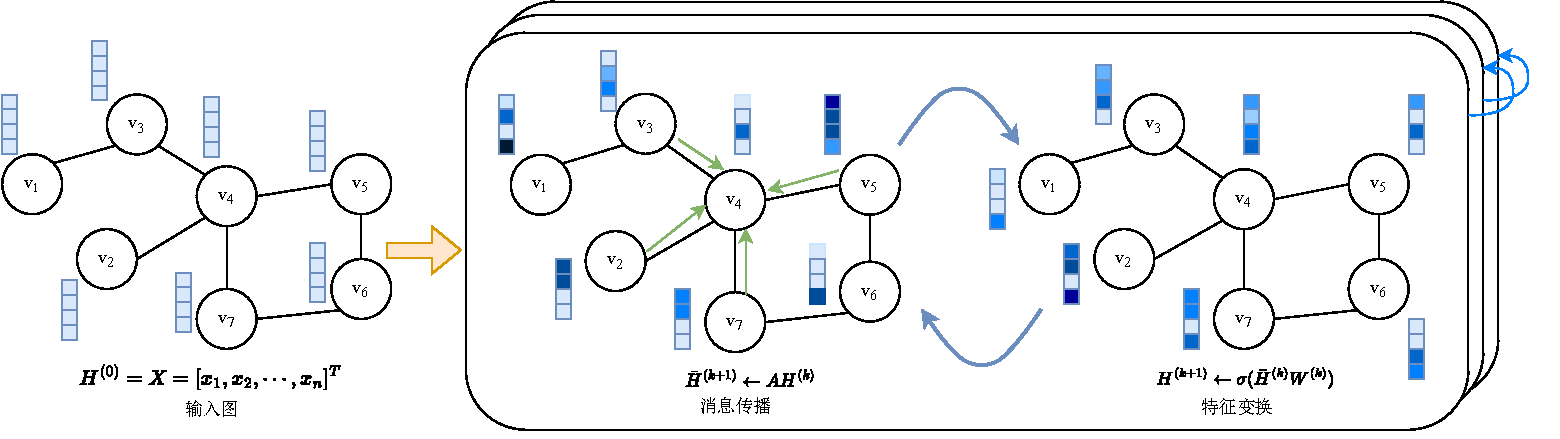
\includegraphics[width=\linewidth]{figure/gcn.drawio.pdf}
    \caption{空域视角下的图神经网络}
    \label{tag:gcn}
\end{figure}

在消息传播阶段,每一个节点都会获取上一层邻居节点的向量。如图~\ref{tag:gcn}~节点 $v_4$ 从邻居节点 $v_2$、$v_3$、$v_5$、$v_7$ 以及自身 $v_4$ 处获得了上一层图卷积的向量。在在特征变换阶段,每一个节点会通过邻居节点进行归一化后,与一个被训练的权重参数相乘。在非线性激活阶段,以上结果将会通过一个非线性函数从而获得非线性表达能力。因此,对于任意的节点 $v_i$而言,在第 $k$ 层获得的特征向量 $h_i^{(k)}$ 可以被定义为:
\begin{gather}
    h_i^{(k)} = f^{(k)}(W^{(k)} \cdot \frac{\sum\limits_{u\in \mathcal{N}(i)} h_u^{k-1}}{|\mathcal{N}(i)|} + B^{(k)} \cdot h_i^{(k-1)})
\end{gather}
其中$\mathcal{N}(i)$ 为节点 $v_i$ 的所有邻居节点,$h_u^{(k-1)}$ 为节点 $v_i$ 的一个邻居节点  $v_u$ 在第 $k-1$ 层的表达,$h_i^{(k-1)}$ 为节点 $v_i$ 在第 $k-1$ 层的表达。$|\mathcal{N}(i)|$ 表示对求和后特征向量进行归一化,以防止向量的数值在经过数层计算后发生尺度上的变化。$B^{(k)}$ 是对节点自身特征的整合操作。

图神经网络通过聚合邻居节点的信息来生成当前节点的表达,其核心思想在于可以通过堆叠多个卷积层来增大单个节点的感受域 (receptive field),从而使节点可以触及多跳邻居的信息,具备高阶连接性。然而,高阶图神经网络会带来过平滑(oversmoothing)的问题\cite{chen_simple_2020}。为了解决这个问题,出现了一些优秀的模型对 GCN 进行改进,例如 GraphSAGE\cite{hamilton_inductive_2018}和 GAT\cite{velickovic_graph_2018}。GraphSAGE 主要从空域切入,通过采样的方式选择一定数量的邻居,避免了计算时将所有邻居节点的参数同时加载到内存造成的内存溢出问题,从而避免了复杂度接近 $O(|V|)$ 的极端情况,并且极大的扩展了图神经网络的尺度,使得图神经网络首次引入到工业推荐系统 Pinterest\footnote{https://www.pinterest.com/} 中。GAT 对邻居节点重要性进行改进,与 GCN 使用邻接矩阵的度作为权重不同,GAT 使用注意力机制来衡量邻居节点相对于目标节点的重要性,从而可以为更加重要的邻居分配更大的权值。

\subsection{基于图神经网络的推荐算法}
在过去几年中,有许多关于图神经网络的推荐算法工作被提出。最直接的原因在于,大多数推荐系统中的数据基本都有图结构,而图神经网络技术已经被证明在各个领域的图表示学习中是非常强大的\cite{zhou_graph_2020}。用户和物品之间的交互数据可以用用户和物品节点之间的二部图~\ref{tag:ui-date}~来表示,其中用户与物品之间的边表示了用户和物品之间的交互。此外,用户与多个物品的交互也可以转换为序列图,表示了物品交互的先后关系~\ref{tag:squ-data}。除此之外,社交网络~\ref{tag:ui-social}。与知识图谱的例子~\ref{tag:ssk-kg}。

\begin{figure}
    \centering
    \begin{subfigure}{0.45\linewidth}
        \centering
        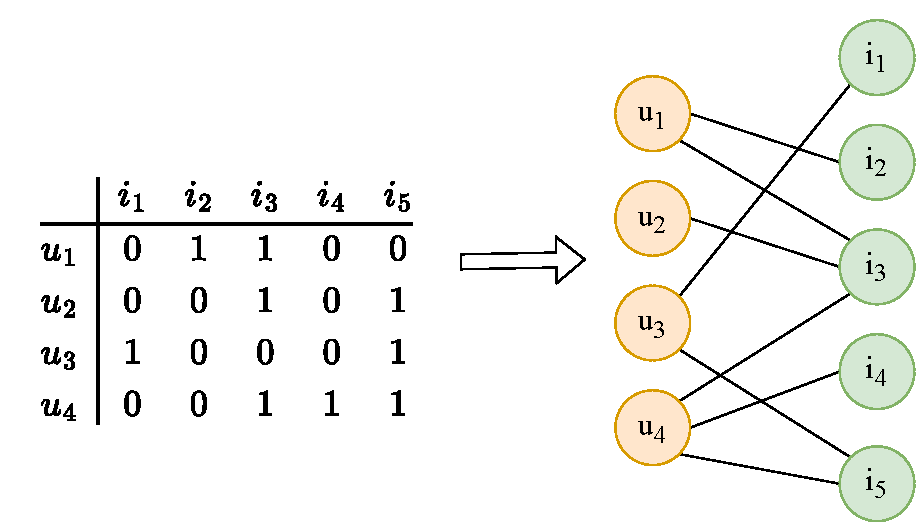
\includegraphics[width=.88\linewidth]{figure/ui-graph.drawio.pdf}
        \caption{用户-物品交互图}
        \label{tag:ui-date}
    \end{subfigure}
    \begin{subfigure}{0.45\linewidth}
        \centering
        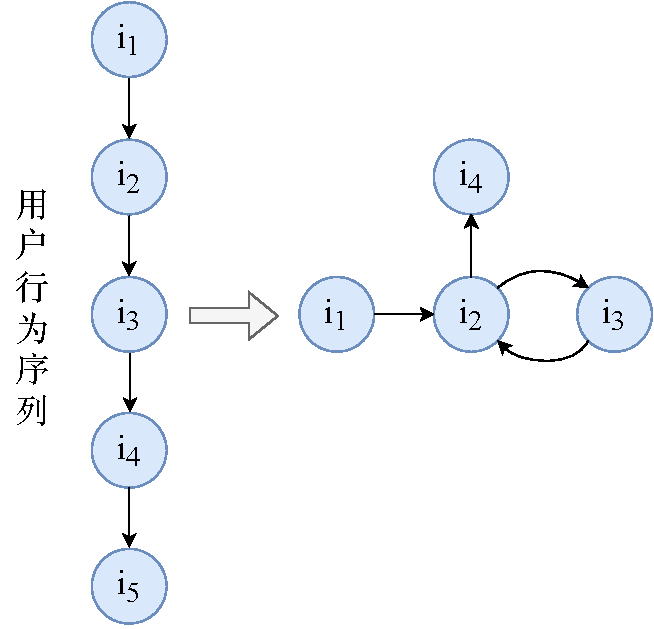
\includegraphics[width=.7\linewidth]{figure/user-seq.drawio.pdf}
        \caption{用户与多个物品交互序列图}
        \label{tag:squ-data}
    \end{subfigure} \\
    \begin{subfigure}{0.45\linewidth}
        \centering
        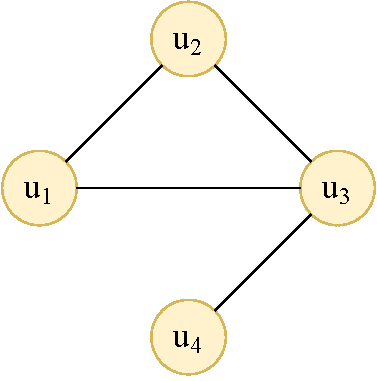
\includegraphics[width=.5\linewidth]{figure/social_graph.drawio.pdf}
        \caption{用户与用户间社交关系图}
        \label{tag:ui-social}
    \end{subfigure}
    \begin{subfigure}{0.45\linewidth}
        \centering
        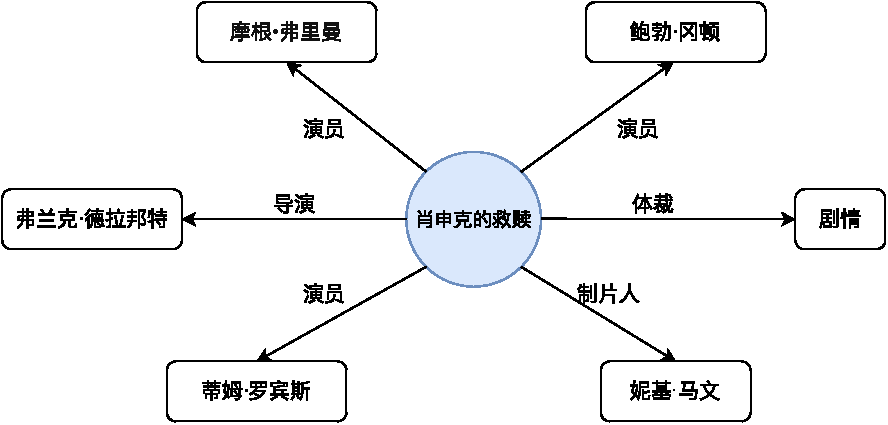
\includegraphics[width=.95\linewidth]{figure/ssk.drawio.pdf}
        \caption{电影肖生克的救赎知识图谱}
        \label{tag:ssk-kg}
    \end{subfigure} 
    \caption{推荐系统中的图数据}
    \label{tag:rs-data}
\end{figure}

虽然利用高阶的协同过滤信息在推荐系统中并不是全新的想法。例如,Koren 等人的 SVD++ 算法\cite{koren_factorization_2008} 结合了被交互的物品等表征来丰富用户表征。另外,Gori 等人的 ItemRank 算法\cite{gori_itemrank_nodate} 通过随机游走算法从物品-物品图中学习表征,并根据用户的偏好对物品进行排名。其中,SVD++ 可以视为是利用一阶邻居来改善用户表征,而 ItemRank 则是利用二阶邻居来改善物品表征。与这些传统算法对比,图神经网络更为灵活,可以更方便地对用户-物品交互中的多跳连接进行建模,并且这些高阶的协同过滤信息已经被证明对推荐系统是有效的\cite{wu_graph_2022}。对于推荐系统而言,其中的图数据通常包括两个方面的信息:

(1)交互信息,记录用户域与物品域之间的交互数据。例如,在标签感知推荐系统中,社会标签数据是一种交互信息。用户使用标签标注物品,这种交互形成了三种边,即用户-标签、物品-标签和用户-物品之间的边;

(2)节点特征,记录某个域自身附带的信息。例如,用户的年龄、性别等信息,物品的标签、评论等信息,这些信息可以作为一类附加信息(side information)在训练时使用。

而基于协同过滤的推荐方法通常只使用第一类信息,这类信息由用户与物品的 ID 特征构成的三元组组成。而并不去使用用户、物品自身的信息。由于图神经网络非常契合推荐系统的数据形式,因此一些算法算法,如 Wang 等人\cite{wang_neural_2019}尝试将完整的图神经网络结构引入推荐系统,提出了 NGCF 模型。但早期的应用图神经网络的算法依照 GCN 相同的消息传播来调优模型的参数:特征变换(feature transformation)、邻居聚合(neighborhood aggregation)与非线性激活(nonlinear activation)。尽管这样的算法展示了图神经网络在推荐系统中大有作为,但更新的研究则证明,完整的图卷积神经网络对于推荐系统而言过于冗余\cite{he_lightgcn_2020}。原始的图卷积神经网络最初是设计用于带有附加特征的图(attributed graph)上的节点分类、整图分类等任务。这类图数据中的节点通常都附带有额外的特征信息作为输入模型的嵌入特征。而在推荐系统中的用户-物品二部图中,每个节点(用户或物品)仅由节点ID作为输入,缺乏额外的语义信息贡献,仅用于区分不同的节点。因此,去除图卷积神经网络中的某些组件,将有助于图神经网络在推荐系统中的应用,He 等人\cite{he_lightgcn_2020} 由此提出了 LightGCN 模型。本小节将继续介绍 NGCF 与 LightGCN 这两个算法。

\subsubsection{NGCF 简介}
对于基于协同过滤的推荐方法,用户、物品的 ID 通常与唯一的一个嵌入表征表示。令用户 $u$ 的表征记为 $e_u^{(0)}$,物品 $i$ 的表征则为 $e_i^{(0)}$。与图卷积神经网络的结构类似,NGCF 在用户-物品二部图上的消息传播可以被定义为:
\begin{equation}
    \begin{aligned}
        e_u^{(k)} = \sigma (W_1 e_u^{(k-1)} + \sum_{i\in\mathcal{N}_u} \frac{1}{\sqrt{|\mathcal{N}_u||\mathcal{N}_i|}}(W_1e_i^{(k-1)} + W_2(e_i^{(k-1)} \odot e_u^{(k-1)} ))) \\
        e_i^{(k)} = \sigma (W_1 e_i^{(k-1)} + \sum_{u\in\mathcal{N}_i} \frac{1}{\sqrt{|\mathcal{N}_i||\mathcal{N}_u|}}(W_1e_u^{(k-1)} + W_2(e_u^{(k-1)} \odot e_i^{(k-1)} )))
    \end{aligned}
\end{equation}
其中,$\sigma(\cdot)$ 为非线性激活函数。$e_u^{(k-1)}$ 和 $e_i^{(k-1)}$ 为用户 $u$ 和物品 $i$ 的嵌入表征经过 $k-1$ 次消息传播得到的嵌入表征。$\mathcal{N}_u$ 为用户 $u$ 交互过的所有物品,$\mathcal{N}_i$ 为物品 $i$ 交互过的所有用户,这些交互关系也可以被视为节点的一阶邻居。$W_1$ 与 $W_2$ 为特征变换所用到的可训练参数。通过 $K$ 次消息传播,最终可以获得 $K+1$ 条用于描述用户的嵌入表征 $(e_u^{(0)},e_u^{(1)},\dots,e_u^{(k)})$ 与 用于描述物品的嵌入表征 $(e_i^{(0)},e_i^{(1)},\dots,e_i^{(k)})$。最终 NGCF 使用拼接(concatenates)的方式,将这些嵌入表征合并,作为最终读出用于推荐的嵌入表征。

NGCF 在很大程度上继承了标准图卷积神经网络的框架,包括使用非线性激活函数 $\sigma(\cdot)$ 和特征变换参数 $W_1$ 和 $W_2$。然而,这些组件已经被证明在基于协同过滤的推荐算法中没有起到作用\cite{he_lightgcn_2020}。对于节点分类、整图分类等任务,每个节点或整个图都拥有丰富的输入特征。例如,在学术引用图中,每个论文节点都可以使用标题和摘要作为输入特征来训练模型\cite{hu_ogb-lsc_2021}。然而,在基于协同过滤的推荐算法中,用户-物品的二部图只包含用于区分节点的 ID 信息。在这种情况下,使用复杂的非线性激活和特征变换无助于学习更优质的特征,甚至会丢失部分协同过滤信息并增加训练难度。

\subsubsection{LightGCN 简介}
比较于 NGCF,LightGCN 去除了特征变换与非线性激活。LightGCN 在用户-物品上的二部图上的消息传播可以被定义为:
\begin{equation}
    \begin{aligned}
        e_u^{k} = \sum_{i\in\mathcal{N}_u} \frac{1}{\sqrt{|\mathcal{N}_u||\mathcal{N}_i|}}e_i^{(k-1)})\\
        e_i^{k} = \sum_{u\in\mathcal{N}_i} \frac{1}{\sqrt{|\mathcal{N}_i||\mathcal{N}_u|}}e_u^{(k-1)})
    \end{aligned}
\end{equation}
其中,用于归一化的$\frac{1}{\sqrt{|\mathcal{N}_u||\mathcal{N}_i|}}$于消息传播在其中得到保留。而 $\sigma(\cdot)$ 非线性激活函数与特征变换 $W_1$ 与 $W_2$ 从 NGCF 的模型被去除。此外,LightGCN 也设计了不同的读出函数,当用户与物品的初始嵌入表征通过 $K$ 次消息传播得到了描述用户的嵌入表征 $(e_u^{(0)},e_u^{(1)},\dots,e_u^{(k)})$ 与用于描述物品的嵌入表征 $(e_i^{(0)},e_i^{(1)},\dots,e_i^{(k)})$ 后,使用简单的加权平均和得到最终用于推荐的嵌入表征。

LightGCN 的优越性在于其简化了 NGCF 中的特征变换和非线性激活函数,从而减少了模型的参数量,避免了过拟合现象,并且保持了模型的高效性。同时,LightGCN能够高效地利用用户-物品交互矩阵中的信息,使得该算法适用于大规模的推荐系统场景。因此,LightGCN 已成为基于协同过滤算法的推荐系统领域的一种重要参考模型,其简洁而有效的设计为推荐系统研究提供了新的思路和方向。

\section{基于轻量化图卷积的标签感知推荐模型 LFGCF}
本节首先提出一种基于轻量化图卷积的标签感知推荐模型 LFGCF,该模型使用简化后的图神经网络,在易于训练的同时提高了推荐性能。
\subsection{模型架构}
在目前主流的图神经网络模型中,如GCN\cite{kipf_gcn_2017} 和 GAT\cite{peter_gan_2017}等模型通常是为节点、边或整图等表征学习而设计的,这些图通常都存在附加特征。具体而言,每个节点都具有输入的嵌入表征,因此需要一个初始特征变换将原始特征转换为统一的格式。接下来,节点上的嵌入表征和其他邻居节点的信息会通过一个聚合函数(aggregation function)进行聚合,最终得到聚合后的嵌入表征。最后,聚合后的嵌入表征通过非线性激活函数更新为新的嵌入表征。然而,在推荐系统中的二部图中,每个节点(包括用户或物品)通常仅拥有唯一的编号,而没有任何有意义的语义信息作为输入特征。在这种情况下,将初始化后的唯一编号嵌入表征作为输入,通过多层特征变换和非线性激活函数来进行推荐系统任务是现代神经网络的关键\cite{he_deep_2015}。然而,这样的操作在图数据上会增加表征学习的难度,从而降低推荐任务的性能\cite{he_lightgcn_2020}。
\begin{gather}
    Top(u, K) = \mathop{argmax}^{(K)}_{i\in \mathcal{I}}(\hat{y}_{u,i})
\end{gather}

本节提出的 LFGCF 如图~\ref{lfgcf}~所示。LFGCF 模型的输入图为社会标注图,且分别对于用户-标签图、物品-标签图进行消息传播操作,由于模型去除了特征变换与非线性激活操作,因此节点的嵌入表征被简单地加权和运算整合。最后,模型使用 BPR 损失函数与基于知识图谱的 TransRT 正则函数联合优化。

\begin{figure}
    \centering
    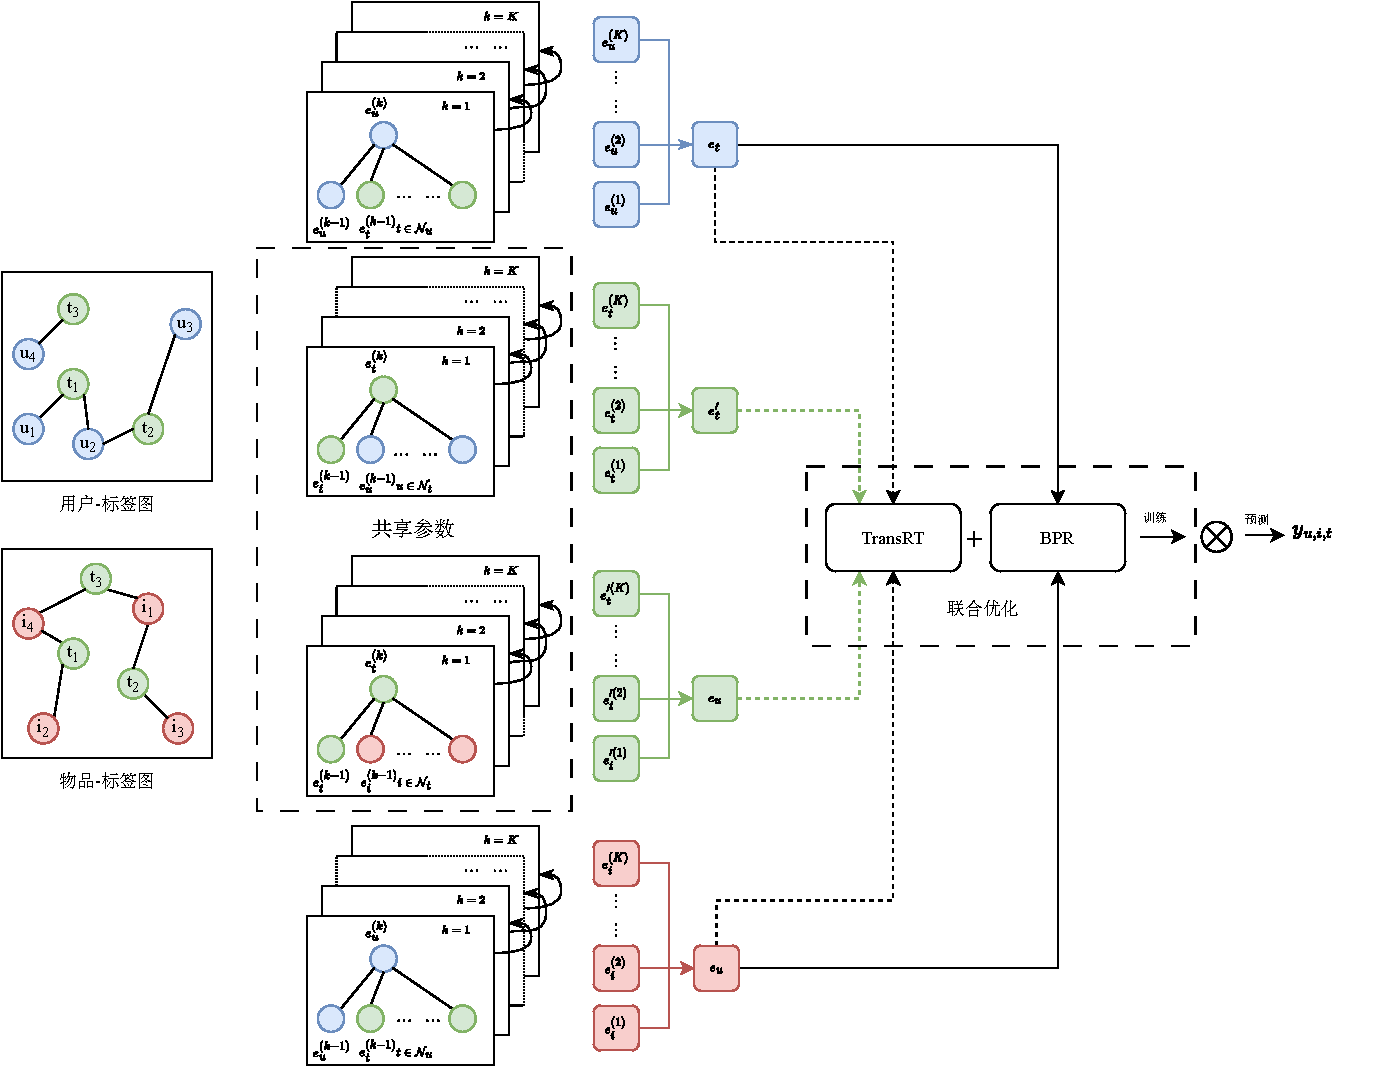
\includegraphics[width=0.88\linewidth]{figure/lfgcf.drawio.pdf}
    \caption{LFGCF 的模型结构}
    \label{lfgcf}
\end{figure}

\subsection{消息传播操作}
一个基础的图神经网络结构会通过消息传递学习到节点的表征\cite{kipf_gcn_2017}。新的节点表征将会从其邻居特征中传播而来。这里的聚合函数可以被定义为:
\begin{equation}
    \begin{aligned}
        e_{u}^{(k+1)} = \mathcal{AGG}(e_{u}^{(k)}, {e_t^{(k)}: t \in \mathcal{N}_{u}}) \\
        e_{i}^{(k+1)} = \mathcal{AGG}(e_{i}^{(k)}, {e_t^{(k)}: t \in \mathcal{N}_{i}})
    \end{aligned}
\end{equation}
其中,$e_{u}, e_{i} \in \mathbf{R}^d$ 分别代表着 $G_{UT}$ or $G_{IT}$ 中的用户和物品节点的表征。此外,$\mathcal{AGG}$ 是邻居聚合函数,其考虑到目标节点与其 $k$ 阶邻居之间的聚合关系。多跳的邻居聚合函数被用于缓解标签感知推荐系统中的稀疏性\cite{chen_tgcn_2020}。许多研究为邻居聚合操作提出了不同的邻居聚合函数,例如在 GIN\cite{chen_tgcn_2020} 中使用的加权和聚合,在 GraphSage\cite{hamilton_graphsage_2017} 中使用的 LSTM 聚合,以及 BGCNN\cite{zhu_bgnn_2020} 中的双线性交互聚合。然而大部分研究都依靠带有复杂的特征变换或者非线形激活的聚合函数,例如 TGCN 中复杂的注意力机制与卷积神经网络设计。尽管这些研究在带有语义特征输入的节点或整图分类任务种取得了非常好的性能,但是标签感知推荐系统仅仅只将编号过的嵌入表征作为输入特征,这样复杂的操作对于 Top-K 推荐任务而言是冗余的。

\subsection{轻量化聚合操作}
本小节对图 $\mathcal{G}_{UT}$ 和图 $\mathcal{G}_{IT}$ 组成的社会标注图进行轻量化后的图神经网络操作。在轻量化的社会标注图卷积神经网络当中,本文主要关注与图卷积神经网络中对于推荐系统最关键的组件。为了轻量化的设计,本文使用了简单的加权和聚合操作,并舍弃了复杂的特征变换以及非线性激活函数。这样的轻量化聚合函数在图 $\mathcal{G}_{UT}$ 可以被定义为:
\begin{equation}
    \begin{aligned}
        e_{u}^{(k+1)} = \sum_{t\in \mathcal{N}_{u}}\frac{1}{\sqrt{|\mathcal{N}_{u}|}\sqrt{|\mathcal{N}_{t}|}}e_t^{(k)} \\
        e_t^{(k+1)} = \sum_{u\in \mathcal{N}_t}\frac{1}{\sqrt{|\mathcal{N}_t|}\sqrt{|\mathcal{N}_{u}|}}e_{u}^{(k)}
    \end{aligned}
\end{equation}
其中对称的归一化项 $\frac{1}{\sqrt{|\mathcal{N}_{u}|}\sqrt{|\mathcal{N}_t|}}$ 服从了标准 GCN 的设计,这是为了避免嵌入表征随着图卷积操作在数量级上的变化。类似于图 $\mathcal{G}_{UT}$ 上的操作,在图 $\mathcal{G}_{IT}$ 种的聚合函数可以被定义为:
\begin{equation}
    \begin{aligned}
        e_{i}^{(k+1)} = \sum_{t\in \mathcal{N}_{i}}\frac{1}{\sqrt{|\mathcal{N}_{i}|}\sqrt{|\mathcal{N}_{t}|}}e_t^{(k)} \\
        e_t^{(k+1)} = \sum_{u\in \mathcal{N}_t}\frac{1}{\sqrt{|\mathcal{N}_t|}\sqrt{|\mathcal{N}_{i}|}}e_{i}^{(k)}
    \end{aligned}
\end{equation}

\subsection{卷积层合并与模型预测}
本文提出的 LFGCF 模型的训练参数仅仅只有第 0 层的嵌入表征。一旦嵌入表征被初始化,后续层便可以用轻量化聚函数合计算得出。经过 K 层轻量化聚合函数计算后,本文提出一个层合并函数,可以进一步合并每一层的嵌入表征并构建出最终的节点表征。层合并函数可以被定义为:
\begin{gather}
    e =\mathcal{COMB}(e^{(k)}:k \in K).
\end{gather}
其中,$\mathcal{COMB}$ 是层的合并函数,它使用了特定节点类型的所有层上的表征。$K$ 是层的数量。不同层的嵌入表征可以捕获到社会标注图中不同的语义信息。例如,第一层通过用户(物品)和标签之间嵌入表征平滑化,第二层则会让用户(物品)和标签存在重叠的嵌入表征变得平滑,更高阶的层可以捕获节点之间更高阶的相似性\cite{wang_neural_2019}。因此,本文并未过度设计特殊的合并函数操作。本文的层合并函数可以被进一步定义为:
\begin{gather}
    e_u= \sum_{k=0}^{K}a_ke_u^{(k)},\quad e_i = \sum_{k=0}^{K}a_ke_i^{(k)}, \quad e_t = \sum_{k=0}^{K}a_ke_t^{(k)}
\end{gather}

其中,$a_k \geq 0$ 贡献了第 K 层的嵌入表征的对于最终嵌入表征的重要性。这个参数可以被作为一个手动调整的超参数,或者一个模型参数在模型训练时自动学习。本文将 $a_k$ 统一的设置成 $1/(K + 1)$,这里的 $K$ 代表了层数。本文设计该层合并函数有两个原因:1) 随着层的提升,嵌入表征将会变得愈加过平滑\cite{li_deeper_2018},因此只使用最后一层最为最终嵌入表征是存在问题的;2) 以不同权重合并不同层的嵌入表征视为是图卷积神经网络中的自连接效应\cite{he_lightgcn_2020}。

最终模型预测可以被定义成用户和物品最终表征之间的内积,这里的得分用于生成最终的推荐结果。:
\begin{gather}
    \hat{y}_{ui} = e_u^{T}e_i
\end{gather}


\subsection{基于知识图谱的嵌入层}
基于知识图谱的表示学习是一种常用的方法,用于缓解知识图谱嵌入中的稀疏性,同时有效地将节点参数化为向量表示,保持图谱的拓扑结构。本文提出了一种基于变换思想的新型知识图谱嵌入方法。具体而言,本文提出了一个新的正则化函数 TransRT,该函数基于在知识图谱中广泛使用的TransR方法\cite{lin_learning_nodate}。具体来说,TransRT 通过优化转换原则 $e_u + e_t \approx e_i$ 来学习每个节点的嵌入。这里,$e_u, e_i, e_t \in \mathbf{R}^d$ 分别是用户$u$、物品 $i$ 和标签 $t$ 的最终嵌入,而 $e_u, e_i$ 代表它们在标签空间的投影表示。因此,对于一条给定的社会标签数据 $(u, t, i)$,其可信度分数可以定义如下:
\begin{gather}
    g(u, t, i) = ||e_u + e_t - e_i||_2^2
\end{gather}
这里,由于 $e_u, e_i, e_t$ 存在于相同的维度空间,但是并不存在于相同的语义空间,因此该分数 $g(u, t, i)$ 越低,说明该大众分类记录越有可能是真实的。

\subsection{模型预测输出与联合优化}
LFGCF 的可训练参数仅仅只有第 0 层的嵌入表征,它合并了社会标注图中的用户、物品和标签与标准的矩阵分解模型的参数复杂度相同。为了获得更好的推荐排序任务,本文使用 BPR 损失函数作为推荐任务的优化函数,该损失函数是一种基于匹配的损失函数,其鼓励被观察到的样本出现的概率要高于没有被观察到,而是被随机采样到的样本。BPR 损失函数可以被定义为:
\begin{gather}
    \mathcal{L}_{rec} = \sum_{(u,i,i') \in \mathcal{O}} -ln(\sigma(\hat{y}_{u,i} - \hat{y}_{u,i'}))
\end{gather}
其中,$\mathcal{O} = \{(u,i,i')|(u,i) \in \mathcal{A},(u,i') \notin \mathcal{A}\}$ 表示配对 $(u,i)$ 在社会标注数据中出现过,而配对 $(u,i')$ 意味着用户 $u$ 和物品 $i'$ 在记录中没有出现过,但是由未观察到的配对中随机采样中获得。

为了训练基于知识图谱的嵌入 TransRT,本文以最小化该似然得分为优化方向:
\begin{gather}
    \mathcal{L}_{T} = \alpha ReLU(g_u(u, t_u, i) - g_i(u, t_i, i)).
\end{gather}
这里的 $\alpha$ 控制着知识图谱正则化的强度,并且 $g_u(u, t_u, i)$ 和 $g_i(u, t_i, i)$ 由社会标注数据计算得到。为了更清楚的展示本文设计的意图,本文简单回顾 BPR 损失函数。BPR 损失通过梯度优化 $\nabla e_u = -\eta (1 - \sigma(\hat{y}_{ui} - \hat{y}_{ui'}))(e_i - e_{i'})$。由于大多数推荐系统都服从长尾分布,$e_u$ 被训练后会越来越与流行的物品 $i$ 的嵌入表征 $e_i$ 相似。这意味着 $e_u$ 和 $e_i$ 会分别从 $G_{UT}$ and $G_{IT}$ 中不同的标签表征嵌入聚合而成。本文的设计确保了标签作为连接用户和物品的桥梁,而不是停留在局部类似的地方,并且通过 TrnasRT 平滑的标签嵌入可以缓解模糊性和冗余性。

为了使推荐的学习参数更有效,并保持大众标注记录之间的正则化关系,本文使用联合学习框架将 Top-K 推荐任务和 TransRT 结合起来。最后,LFGCF 的总目标函数定义如下:
\begin{gather}
    \mathcal{L} = \mathcal{L}_{rec} + \mathcal{L}_{T} + \gamma ||\Theta||_2.
\end{gather}
这里,$\gamma$ 控制着正则化的强度。本文使用 Adam\cite{kingma_adam_2014} 优化$\mathcal{L}_{rec}$ 和 $\mathcal{L}_{T}$ 并在小批量策略进行训练。最后,本文使用早停策略来防止模型被过度训练。

\section{本章小结}
本章深入介绍了图神经网络,并从空间域和矩阵两个时间理解消息传播的本质。接着介绍了 NGCF 和 LightGCN 两个推荐模型,其中 LightGCN 由于使用了轻量化的图神经网络,从而对比 NGCF 有着显著的性能提升。之后,本章提出了 LFGCF。模型由轻量化的社会标注图卷积神经网络与基于知识图谱的标签关系映射两个核心模块组成,最后使用 Top-K 推荐任务多任务学习优化目标函数,得到最后的推荐模型。
